\section{Context}

%\subsection{Context of the projet}

\begin{frame}{Project initiation}

  \begin{block}{Compagnie Nationale du Rhône (CNR)}
    \begin{itemize}
      \item 1\textsuperscript{st} producer of exclusively renewable energy in France
      \item 18 hydroelectric facilities on the Rhône River (3000 MW)
      \item CNR Engineering Departement (for CNR and third party)
    \end{itemize}
  \end{block}

  \pause

  \begin{block}{Needs and purpose}
    \begin{itemize}
      \item Develop non-existing features, customize it for modeller needs
      \item Automate and chain Telemac post-processing tasks
      \item Do not substitute for common post-processing graphical softwares
    \end{itemize}
  \end{block}

\end{frame}

\begin{frame}{Python Telemac Tools}


\begin{columns}[onlytextwidth]
  \begin{column}{0.4\textwidth}

    \begin{block}{Developement Guidelines}<1->
      \begin{itemize}
        \item extensible
        \item customizable
        \item accessible, easy to use
        \item robustness
        \item open-source
      \end{itemize}
    \end{block}
    \includegraphics<1>[width=0.95\textwidth]{schemas/PyTelTools_organization_empty.pdf}
    \includegraphics<2->[width=0.95\textwidth]{schemas/PyTelTools_organization.pdf}
  \end{column}

  \begin{column}{0.55\textwidth}

    \begin{block}<2->{Implementation overview}
      \begin{itemize}
        \item \textbf{core}
          \begin{itemize}
            \item parsers, base classes, ...
            \item mathematical and spatial calculations
          \end{itemize}
        \item Command Line Interface (\textbf{CLI})
          \begin{itemize}
            \item multiple arguments
            \item easily adapted, snippets (being implemented)
          \end{itemize}
        \item Graphical User Interface (\textbf{GUI})
          \begin{itemize}
            \item classic interface
            \item \textbf{Workflow} : automate, chain and monitor tasks
          \end{itemize}
      \end{itemize}
    \end{block}

  \end{column}
\end{columns}

\end{frame}

%% \begin{columns}[onlytextwidth]
%%   \begin{column}{0.65\textwidth}
%%     \begin{block}{Commande Line Interface (cli)}
%%       \begin{itemize}
%%         \item a
%%         \item b
%%       \end{itemize}
%%     \end{block}
%%   \end{column}
%%   \begin{column}{0.3\textwidth}
%%     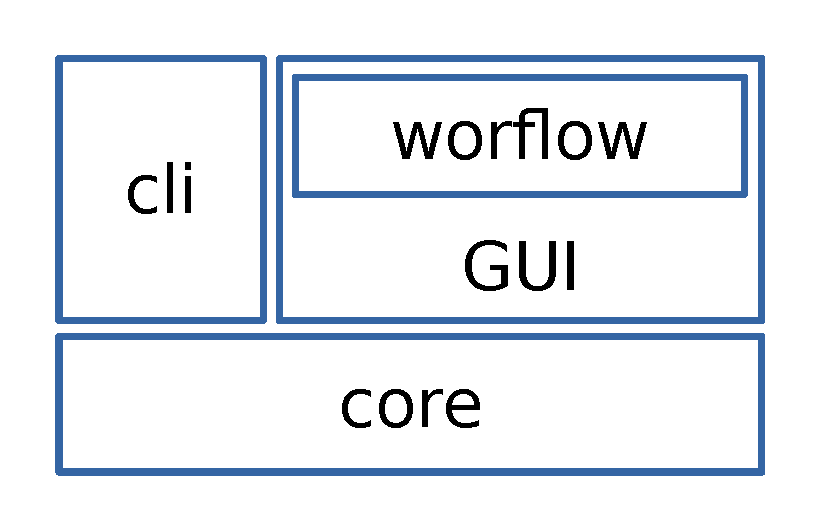
\includegraphics[width=0.95\textwidth]{schemas/PyTelTools_organization.pdf}
%%   \end{column}
%% \end{columns}


\begin{frame}{Documentation and installation}

  \begin{block}{Installation}
    \begin{itemize}
      \item Prerequisites: Python3
      \item Packages: see \href{https://github.com/CNR-Engineering/PyTelTools/blob/master/requirements.txt}{requirements.txt}  (numpy, matplotlib, PyQt5, ...)
      \item Installation procedure:
    \end{itemize}

    \inputminted[fontsize=\tiny,xleftmargin=1.5cm]{bash}{installation.sh}

  \end{block}

  \begin{block}{Documentations}
    \begin{itemize}
      \item User: \url{https://github.com/CNR-Engineering/PyTelTools/wiki}
      \item Developper: \url{https://cnr-engineering.github.io/PyTelTools}
    \end{itemize}
  \end{block}

\end{frame}


%% \begin{python}
%% import numpy as np

%% def incmatrix(genl1,genl2):
%%     m = len(genl1)
%%     n = len(genl2)
%%     M = None #to become the incidence matrix
%%     VT = np.zeros((n*m,1), int)  #dummy variable
%% \end{python}
  %\begin{lstlisting}

%% \begin{lstlisting}[language=html]

%% \begin{minted}[mathescape,
%%                linenos,
%%                numbersep=5pt,
%%                gobble=2,
%%                frame=lines,
%%                framesep=2mm]{python}
%% import numpy as np

%% def incmatrix(genl1,genl2):
%%     m = len(genl1)
%%     n = len(genl2)
%%     M = None #to become the incidence matrix
%%     VT = np.zeros((n*m,1), int)  #dummy variable
%% \end{minted}

%% \begin{lstlisting}
%% Put your code here.
%% \end{lstlisting}

%\lstinputlisting[language=Python]{filename.py}

% https://tex.stackexchange.com/questions/53998/beamer-how-text-wrapping-around-a-graphic-right-aligned
%% \begin{frame}{Folientitel}

%% \begin{minipage}[0.2\textheight]{\textwidth}
%% \begin{columns}[T]
%% \begin{column}{0.8\textwidth}
%% \begin{itemize}
%% \item Punkt 1 = text blah blah foo bar, text blah blah foo bar, text blah blah foo bar
%% \item Punkt 2= text blah blah foo bar, text blah blah foo bar, text blah blah foo bar
%% \item Punkt 3= text blah blah foo bar, text blah blah foo bar, text blah blah foo bar
%% \end{itemize}
%% \end{column}
%% \begin{column}{0.2\textwidth}
%% 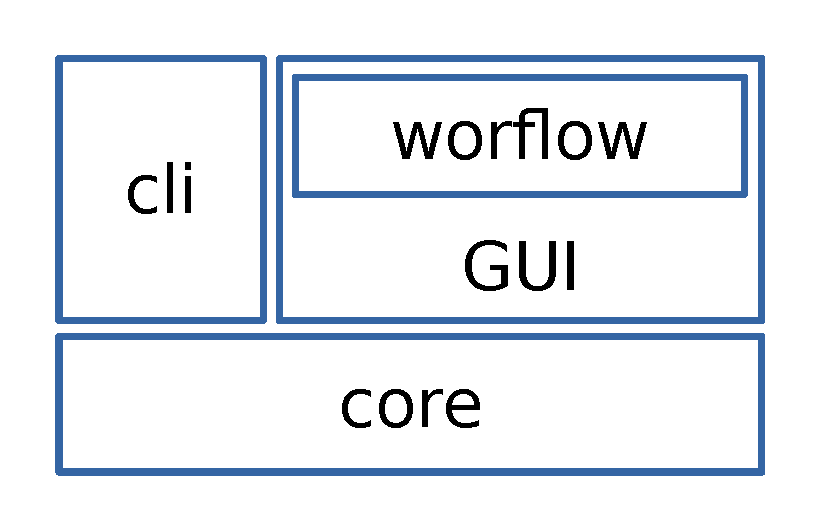
\includegraphics[width=2.5cm]{schemas/PyTelTools_organization.pdf}
%% \end{column}
%% \end{columns}
%% \end{minipage}

%% \begin{itemize}
%% \item Punkt 1 = text blah blah foo bar, text blah blah foo bar, text blah blah foo bar
%% \item Punkt 2= text blah blah foo bar, text blah blah foo bar, text blah blah foo bar
%% \item Punkt 3= text blah blah foo bar, text blah blah foo bar, text blah blah foo bar
%% \end{itemize}
%% \end{frame}
